\documentclass{article}
\usepackage[utf8]{inputenc}
\usepackage[margin = 0.8in]{geometry}
\usepackage{graphicx}
\usepackage{amsmath, amssymb}
\usepackage{subcaption}
\usepackage{multirow}
\usepackage{mathtools}
\usepackage{float}


\title{RBE549 - Midterm Exam}
\author{Keith Chester}
\date{Due date: October 16, 2022}

\begin{document}
\maketitle

\section*{Problem 1}

In this problem we are presented with a Hough transform problem, wherein $x$, $y$, $b$, and $m$ are positive or negative real numbers. 2 points are given in $(m,b)$ space by $P_1: (m,b)=(0.5,4)$ and $P_2: (m,b)=(0.9,0)$.

\subsection*{A}

What line $L_1$ in $(m,b)$ space through $P_1$ and $P_2$?

We can set the line equation ($y=mx+b$) for $P_1$ and $P_2$ equal to eachother to solve this.

\begin{equation}
    P_1 = P_2
\end{equation}

\begin{equation}
    0.5x+4 = 0.9x + 0
\end{equation}

\begin{equation}
    4 = 0.4x
\end{equation}

\begin{equation}
    10 = x
\end{equation}

\noindent ...and then we plug in $x$ to solve for $y$:

\begin{equation}
    0.5(10)+4 = y
\end{equation}

\begin{equation}
    y = 9
\end{equation}

\noindent ...thus the equation for $L_1$, a line that passes through points $P_1$ and $P_2$, is $b = -10m + 9$.

\subsection*{B}

The point $P_3$ in $(x,y)$ space that corresponds to line $L_1$ is the point $(10,9)$, as calculated above in part $A$. We can also just deduce it from our solved equation mentioned in $A$ - specifically that since $y=mx+b$ for $b=-mx+y$, and we stated that $b=-10m+9$, we can also deduce that $(x,y)=(10,9)$.

\subsection*{C}

Since it is a horizontal line, which means the slope $m$ must be $m=0$, we now know that the resulting point, $P_4$, must fall along the line we calculated earlier, $L_1$, specifically where $m=0$, or the vertical axis of $(m,b)$ space. Thus we can solve:

\begin{equation}
    b = -10m + 9
\end{equation}

\begin{equation}
    b = -10*0 + 9
\end{equation}

\begin{equation}
    b = 9
\end{equation}

\noindent ...thus we know that $P_4$ will fall on $(m,b)=(0,9)$. This means that the equation for $L_2$ is $y=9$.

\section*{Problem 2}

In this problem we are aiming to discover a structuring element $SE$ such that $II\bigoplus SE =OI$

\subsection*{A}

A $3x3$ structing element SE that satisfies the given $II$ and $OI$ would be:

\begin{equation}
    \begin{tabular}{ | c | c | c | }
        \hline
        1 & 0 & 1 \\
        \hline
        0 & \textbf{0} & 0 \\
        \hline
        1 & 0 & 1 \\
        \hline
    \end{tabular}
\end{equation}

\noindent ...where the central $0$ is the point of origin for the $SE$.

\subsection*{B}

Another structuring element $SE_2$ can satisfy $II\bigoplus SE_2 = II$ but $SE\neq SE_2$, where again the central value (now a $1$) is the point of origin::

\begin{equation}
    \begin{tabular}{ | c | c | c | }
        \hline
        1 & 0 & 1 \\
        \hline
        0 & \textbf{1} & 0 \\
        \hline
        1 & 0 & 1 \\
        \hline
    \end{tabular}
\end{equation}


\section*{Problem 3}

In this problem we are solving equations having to do with image focus and lenses.

\subsection*{A}


In this problem, we attempt to prove with similar triangles that:

\begin{equation}
    \frac{1}{-z_0} + \frac{1}{z_c} = \frac{1}{f}
\end{equation}

First, we look at the original diagram provided. I have added markers for the lengths ($z_0$ and $z_c$) assigned to their lengths, and marked the two lengths of $f$ to its distance from the center of the lens.

\begin{figure}[H]
    \centering
    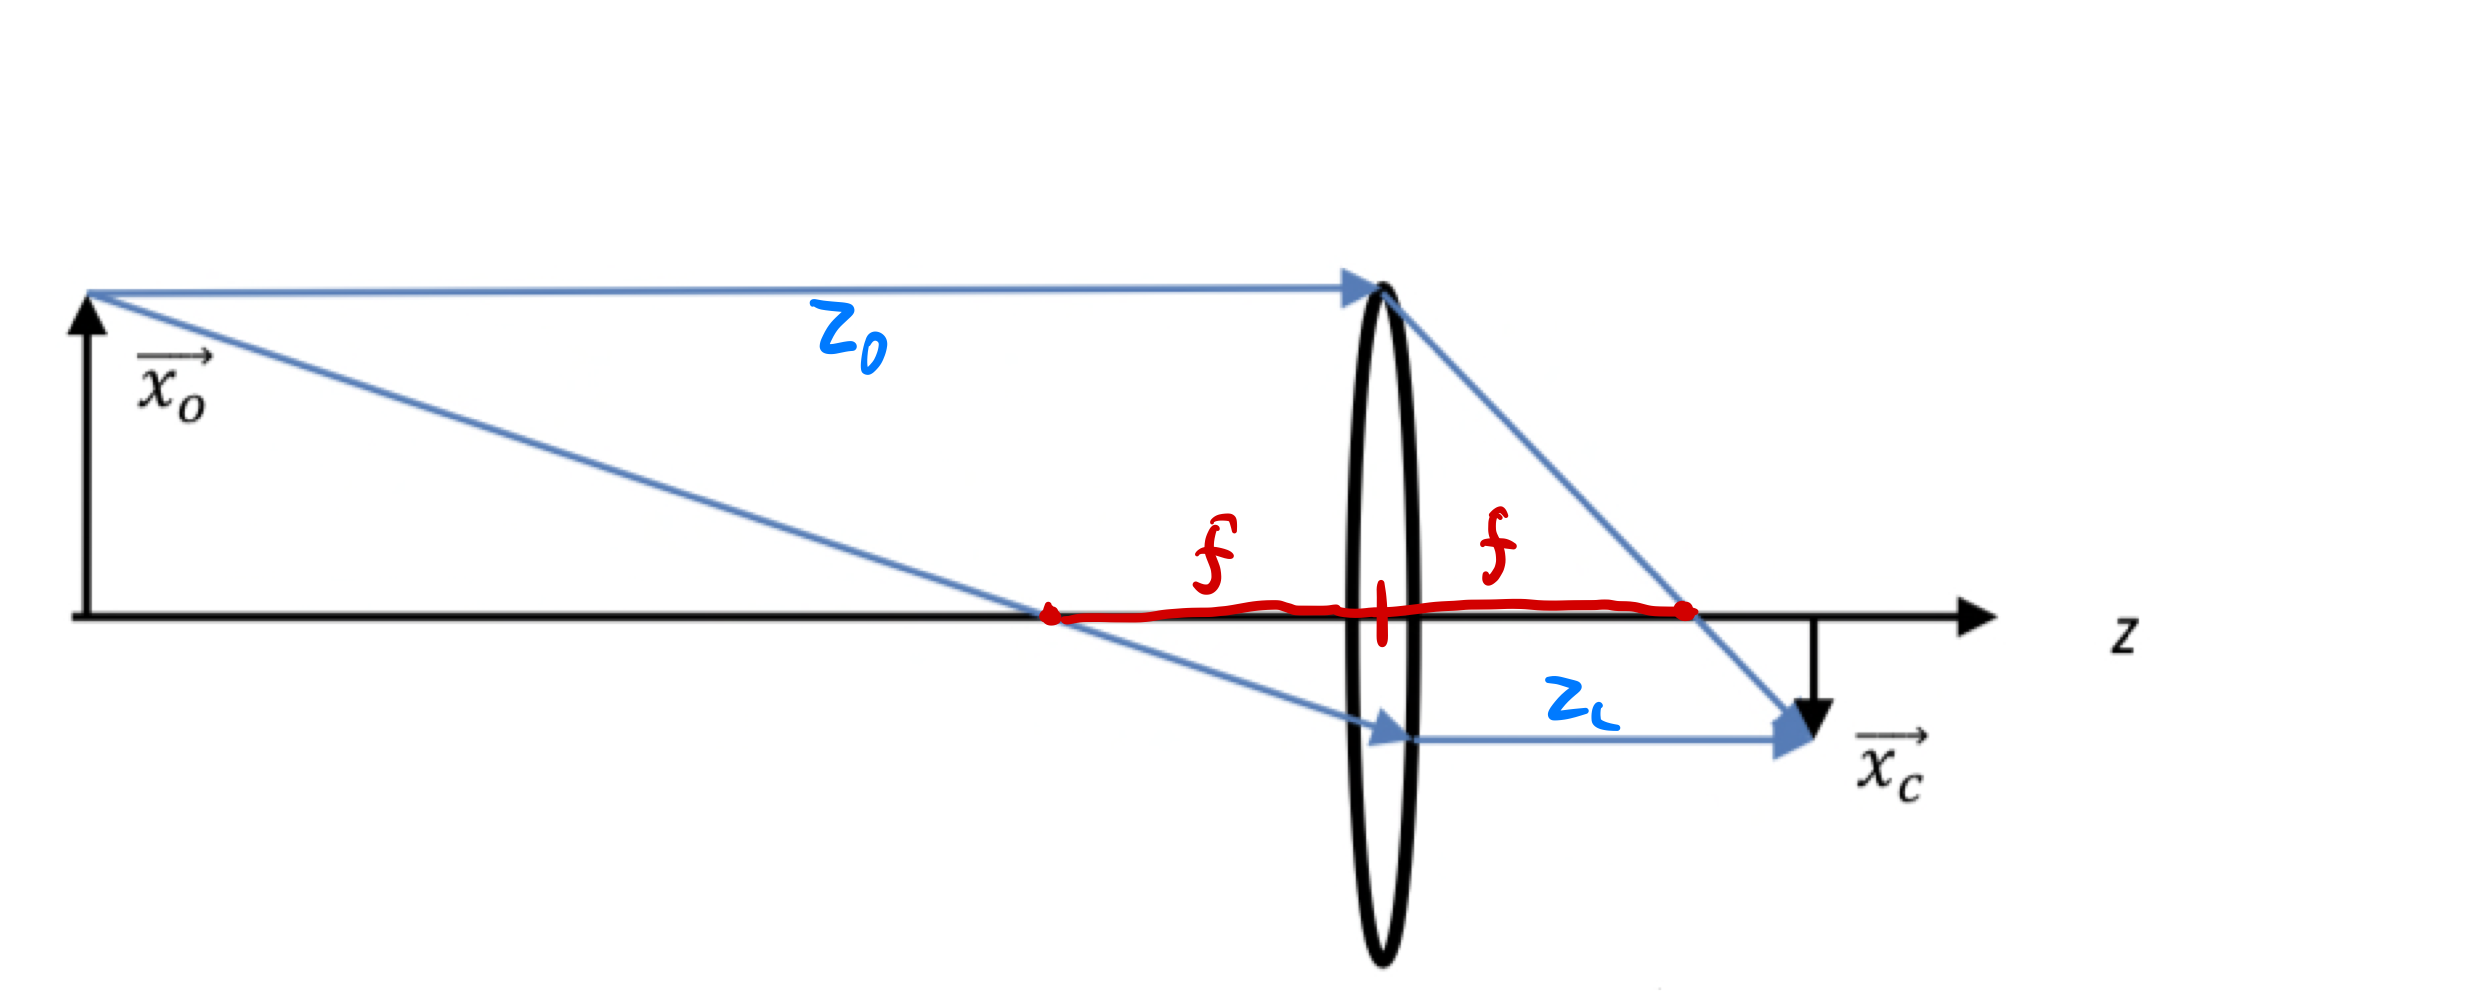
\includegraphics[width = 0.7\textwidth]{imgs/prob_3.png}
    \caption{Thin Lens Diagram}
    \label{fig:prob1}
\end{figure}

We will note that the triangle provided by $z_0$ and be represented on the other side of the lens by flipping it along the lens as an axis. From there we can begin to mark angles.

\begin{figure}[H]
    \centering
    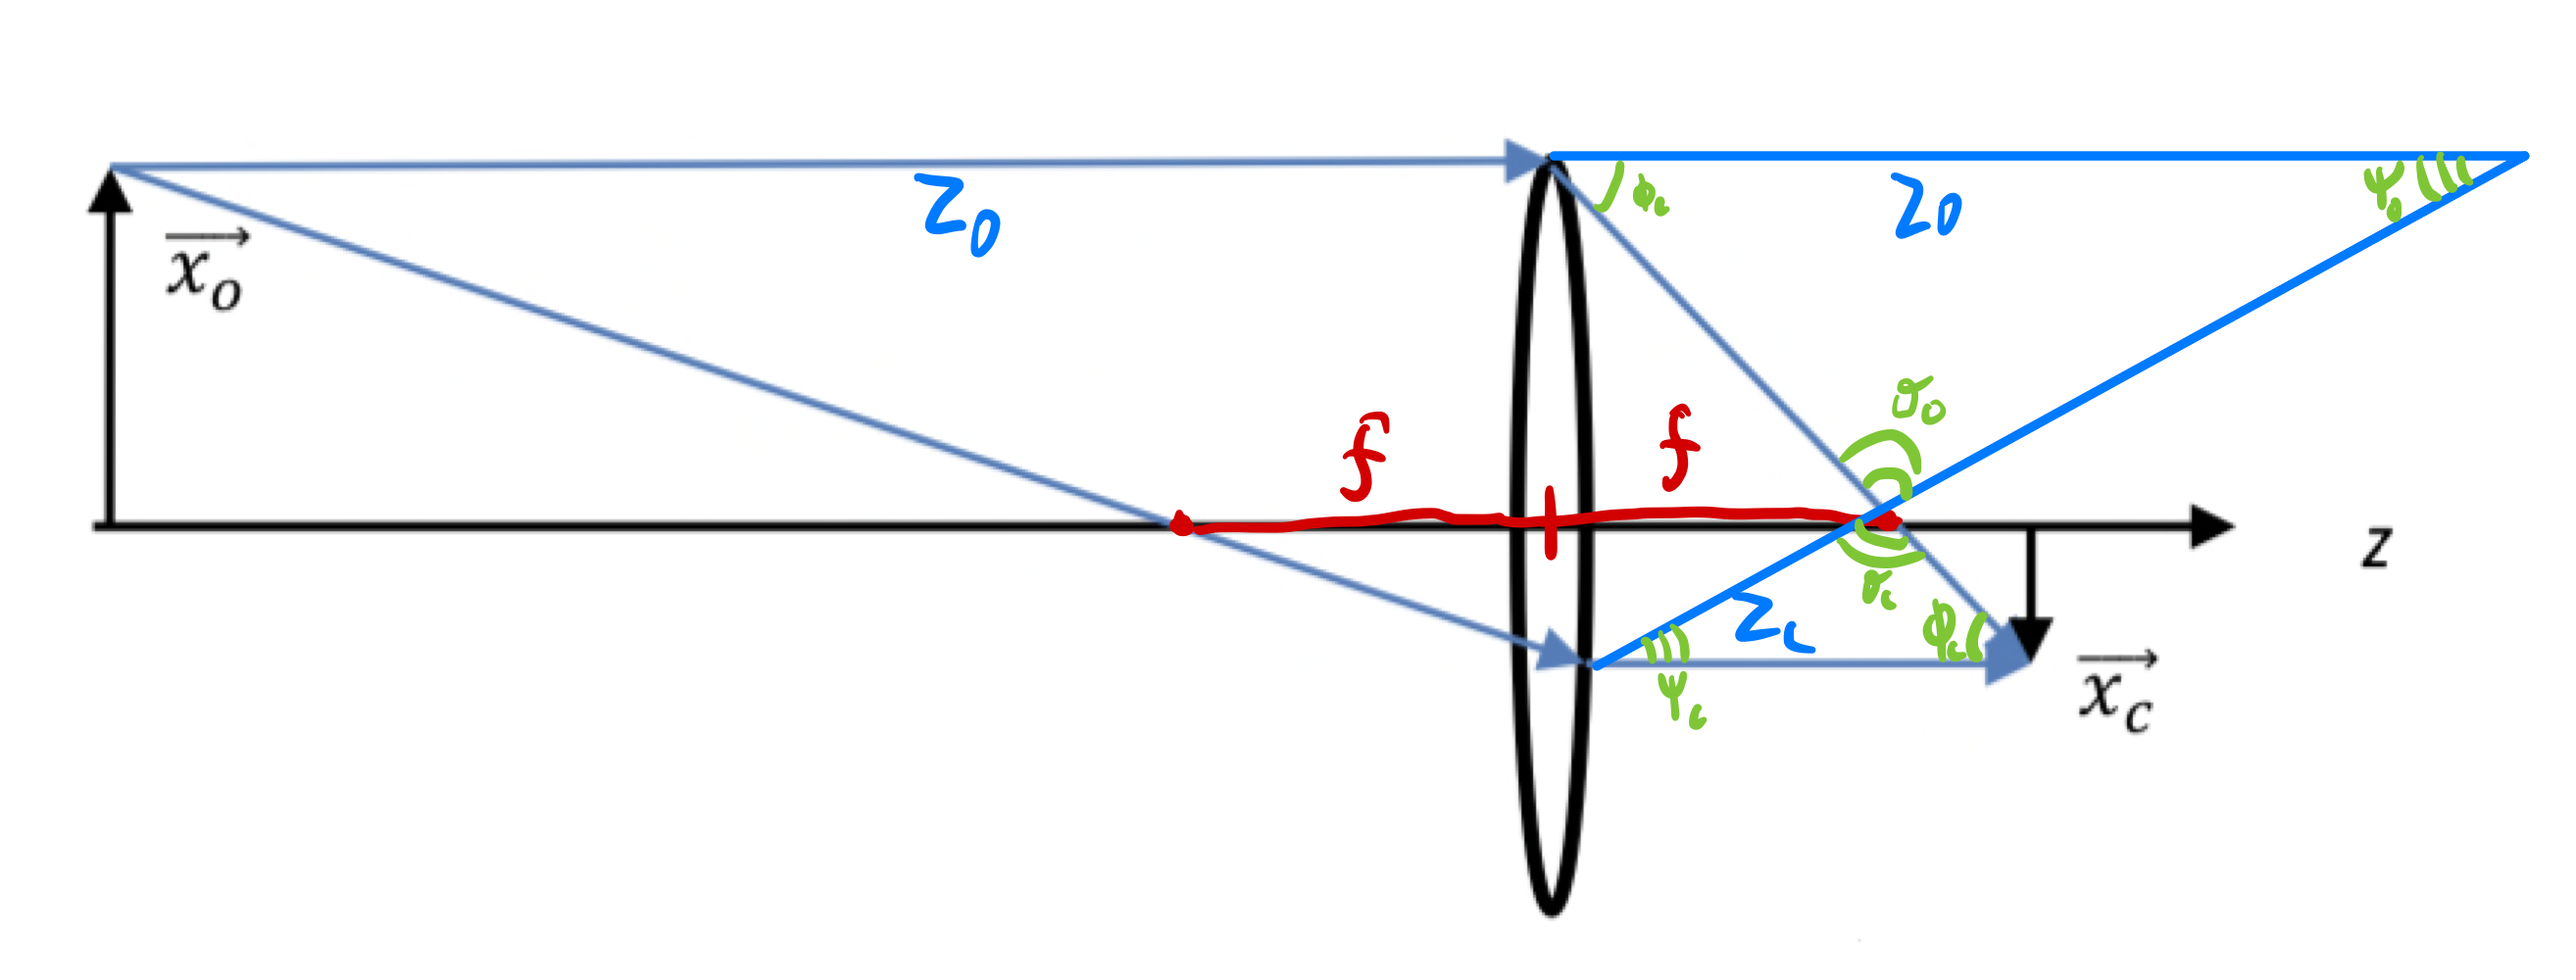
\includegraphics[width = 0.7\textwidth]{imgs/prob_3_expanded.png}
    \caption{Thin Lens Diagram Expanded}
    \label{fig:prob1_expanded}
\end{figure}

Because the $z$ access, $z_c$, and $z_0$ are parallel lines, we can thus know that opposite angles of lines crossing them are equivalent. Thus we see that $\phi_c$ and $\phi_0$ are equivalent and marked as such. Thesame goes for $\psi_c$ and $\psi_0$, as marked.  Since the lines passing through the focal point $f$ is rom parallel lines and continuous, we can also determine that $\theta_0$ and $\theta_c$ are also equivalent.

With this, we know that these are similar triangles, and can begin to form ratios to represent the relationships. Thus we have:

\begin{equation}
    \frac{-z_0}{z_c} = \frac{f}{z_c - f}
\end{equation}

From here we can perform algebra to isolate the variables into a manner that is closer to what we sought to originally prove:

\begin{equation}
    -z_0 z_c - z_0 f = z_c f
\end{equation}

\begin {equation}
    -z_0 z_c = z_c f - z_0 f
\end{equation}

\begin{equation}
    -z_0 z_c = f (z_c - z_0)
\end{equation}

\begin{equation}
    \frac{-z_0 z_c}{f} = z_c - z_0
\end{equation}

\begin {equation}
    \frac{1}{f} = \frac{z_c - z_0}{-z_0 z_c}
\end{equation}

\begin{equation}
    \frac{1}{f} = \frac{z_c}{-z_0 z_c} + \frac{z_0}{z_0 z_c}
\end{equation}

\begin{eqnarray}
    \frac{1}{f} = \frac{1}{-z_0} + \frac{1}{z_c}
\end{eqnarray}

\subsection*{B}

In this problem we are tasked with finding the number of receptors on which the image of Mars falls while looking up into the night sky. We say that a human eyeball has a radius of $12mm$ and contains roughly $1.5\times10^8$ receptors. We assume that the receptors are uniform across a $160^\circ$ partial sphere in the back of our eye. The planet of Mars has a $4\times10^3km$ radius with an average distance of $2.25\times10^8km$. We use an $f$ focal value equal to the eye's diameter ($24mm$).

To solve this, first we use similar triangles using a lens diagram (similar to the one provided for the question in $3A$); this allows us to determine the size of the image of Mars on our eye.

\begin{equation}
    \frac{z_0}{z_c} = \frac{h_0}{h_1}
\end{equation}

\noindent In this we have $z_0$ as the distance from Mars to our eye, and $h_0$ the width of Mars, and $h_i$ is the size of the image of Mars on our eye. We need to solve for $z_c$ before we can figure out $h_1$, so to do this we look at the equation utilized earlier:

\begin{equation}
    \frac{1}{-z_0}+\frac{1}{z_c}=\frac{1}{f}
\end{equation}

\begin{equation}
    \frac{1}{-2.25\times10^8km}+\frac{1}{z_c}=\frac{1}{24mm}
\end{equation}

\begin{equation}
    \frac{1}{z_c} \approx 83.33 + 4.44\times10^{-9}
\end{equation}

\begin{equation}
    z_c \approx 0.024 \approx 24 mm
\end{equation}

Now we can determine the size of the image of Mars on our eye:

\begin{equation}
    \frac{z_0}{z_c} = \frac{h_0}{h_1}
\end{equation}

\begin{equation}
    \frac{2.25\times10^8km}{12mm} = \frac{8,000km}{h_1}
\end{equation}

\begin{equation}
    h_1 = 8.53\times10^{-7} m = 8.53\times10^{-4}
\end{equation}

\noindent ...which is an incredibly tiny size. So let's figure out how many receptors we have per square $mm$ of our eye. First we need to find the area of a spherical cap, such that we can determine the average number of receptors per mm in the eye. We know that the area of a spherical cap ($S$) is:
% S = 2 *pi* r * h where h=r-sqrt(r^2 - a^2) and a=rcos(10degrees)
\begin{equation}
    S = 2rh\pi
\end{equation}

\noindent ...where $h$ is equal to:

\begin{equation}
    h=r - \sqrt{r^2 - a^2}
\end{equation}

\noindent ...but because of the partial sphere, a is not straight but rather angled to reach the $160^\circ$; thus we have an actual interior angle of $80^\circ$, so $a=r*\cos(10^\circ)$

\begin{equation}
    h = 12mm-\sqrt{(12mm)^2 - (12mm * \cos(10^\circ))^2}
\end{equation}

\begin{equation}
    h \approx 0.00992 \approx 9.92mm 
\end{equation}

\noindent Now that we have $h$, we can solve for $S$:

\begin{equation}
    S = 2rh\pi = 2*12mm*9.92mm*\pi \approx 747.95 mm^2
\end{equation}

\noindent Since we know that there are approximately $1.5\times10^8$ receptors, we can use a ratio to get the approximate receptors per $mm$, or $r_{mm}$:

\begin{equation}
    \frac{1mm^2}{r_{mm}} = \frac{747.95mm^2}{1.5\times 10^8}
\end{equation}

\begin{equation}
    r_{mm} \approx 200,548
\end{equation}

\noindent Now that we know the number of receptors per mm, we need to find the area that the Mars image sits on. With an image height of $8.53\times10^{-7}$, which means a radius of half that, or $4.27\times10^{-7}$, which is our $a$. Using the area formulas we used earlier:

\begin{equation}
    h = r - \sqrt{r^2 - a^2} = 12mm - \sqrt{(12mm)^2 - (4.27\times10^{-4})^2} = 7.60\times10^{-9}
\end{equation}

\begin{equation}
    S = 2 \pi r h = 2 \pi (12mm) {7.11\times10^{-7}mm} = 5.73\times10^{-7} mm^2
\end{equation}

\noindent So this area times our known receptors per $mm$:

\begin{equation}
    x_{receptors} = 200,548 \times 5.73\times10^{-7} = 0.115
\end{equation}

\noindent ...and now, we have $\approx 0.115$ receptors seeing the image of Mars - which is why you can't see Mars with your naked eye on a clear night when it's at the average distance.

\section*{Problem 4}

In this problem we have an image which has two background objects and background pixels with brightness values that are distributed according to the Rayleigh distribution with parameters $\sigma_b$, $\sigma_{o1}$, and $\sigma_{o2}$ with $0<\sigma_b < \sigma_{o1} < \sigma_{o2}$. The probability of having brightness $k$ is given by:

\begin{equation}
    P_b(k) = \frac{k}{\sigma^2_b}e^{\frac{-k^2}{2\sigma^2_b}},
    P_{o1}(k) = \frac{k}{\sigma^2_{o1}}e^{\frac{-k^2}{2\sigma^2_{o1}}},
    P_{o2}(k) = \frac{k}{\sigma^2_{o2}}e^{\frac{-k^2}{2\sigma^2_{o2}}}
\end{equation}

We wish to find the decision rule that maximizes the probability of a correct decision. We'll use two thresholds - specifically first we check if the given pixel is ${b}$ or $o1$. Then a second threshold, which we'll calculate as well, is ${o2}$.

\begin {equation}
    \frac{1}{\sqrt{2\pi}\sigma_{o1}}e^{\frac{-(x-\mu)^2}{2\sigma^2_{o1}}}
    >
    \frac{1}{\sqrt{2\pi}\sigma_b}e^{\frac{-(x-\mu)^2}{2\sigma^2_b}}
\end{equation}

First we will try to isolate our terms by taking the natural log. Since $ln(ab) = ln(a) + ln(b)$ and $ln(\frac{a}{b}) = ln(a) - ln(b)$...:

\begin{equation}
    \ln(1) - \ln(\sqrt{2\pi}\sigma_{o1}) + \frac{-(x-\mu)^2}{2\sigma^2_{o1}}
    >
    \ln(1) - \ln(\sqrt{2\pi}\sigma_b) + \frac{-(x-\mu)^2}{2\sigma^2_b}
\end{equation}

\begin{equation}
    \ln(\sigma_b) - \ln(\sigma_{o1}) > \frac{-(x-\mu)^2}{2\sigma^2_{o1}} - \frac{-(x-\mu)^2}{2\sigma^2_b}
\end{equation}

\begin{equation}
    \ln(\sigma_b) - \ln(\sigma_{o1}) > \frac{((x-\mu)^2 2\sigma_b^2 - ((x-\mu)^2 2\sigma_{o1}^2 }{2\sigma^2_{o1}2 \sigma^2_b2}
\end{equation}

\begin{equation}
    (\ln(\sigma_b) - \ln(\sigma_{o1})) (2\sigma^2_{o1}2 \sigma^2_b2)  > ((x-\mu)^2 2\sigma_b^2) - ((x-\mu)^2 2\sigma_{o1}^2)
\end{equation}

\begin{equation}
    \frac{(\ln(\sigma_b) - \ln(\sigma_{o1})) (2\sigma^2_{o1}2 \sigma^2_b2)}{\sigma_b^2 - \sigma_{o1}^2} > (x - \mu)^2
\end{equation}

...and finally we can finalize this result by taking the square root of above, resulting in:

\begin{equation}
    \sigma_b \sigma_{o1} \sqrt{2\frac{\ln(\sigma_b) - \ln(\sigma_{o1})}{\sigma_b^2 - \sigma_{o1}^2}} > \vert x - \mu \vert
\end{equation}

We will redo this process again for the $o2 > o1$ threshold.

\begin {equation}
    \frac{1}{\sqrt{2\pi}\sigma_{o2}}e^{\frac{-(x-\mu)^2}{2\sigma^2_{o2}}}
    >
    \frac{1}{\sqrt{2\pi}\sigma_{o1}}e^{\frac{-(x-\mu)^2}{2\sigma^2_{o1}}}
\end{equation}


\begin{equation}
    \ln(1) - \ln(\sqrt{2\pi}\sigma_{o2}) + \frac{-(x-\mu)^2}{2\sigma^2_{o2}}
    >
    \ln(1) - \ln(\sqrt{2\pi}\sigma_{o1}) + \frac{-(x-\mu)^2}{2\sigma^2_{o1}}
\end{equation}

\begin{equation}
    \ln(\sigma_{o1}) - \ln(\sigma_{o2}) > \frac{-(x-\mu)^2}{2\sigma^2_{o2}} - \frac{-(x-\mu)^2}{2\sigma^2_{o1}}
\end{equation}

\begin{equation}
    \ln(\sigma_{o1}) - \ln(\sigma_{o2}) > \frac{((x-\mu)^2 2\sigma_{o1}^2 - ((x-\mu)^2 2\sigma_{o2}^2 }{2\sigma^2_{o2}2 \sigma^2_{o1}2}
\end{equation}

\begin{equation}
    (\ln(\sigma_{o1}) - \ln(\sigma_{o2})) (2\sigma^2_{o2}2 \sigma^2_{o1}2)  > ((x-\mu)^2 2\sigma_{o1}^2) - ((x-\mu)^2 2\sigma_{o2}^2)
\end{equation}

\begin{equation}
    \frac{(\ln(\sigma_{o1}) - \ln(\sigma_{o2})) (2\sigma^2_{o2}2 \sigma^2_{o1}2)}{\sigma_{o1}^2 - \sigma_{o2}^2} > (x - \mu)^2
\end{equation}

...and finally we can finalize this result by taking the square root of above, resulting in:

\begin{equation}
    \sigma_b \sigma_{o2} \sqrt{2\frac{\ln(\sigma_{o1}) - \ln(\sigma_{o2})}{\sigma_{o1}^2 - \sigma_{o2}^2}} > \vert x - \mu \vert
\end{equation}



\end{document}
